\documentclass{standalone}

\usepackage{amsmath}
\usepackage{tikz}
\usetikzlibrary{math}

\begin{document}

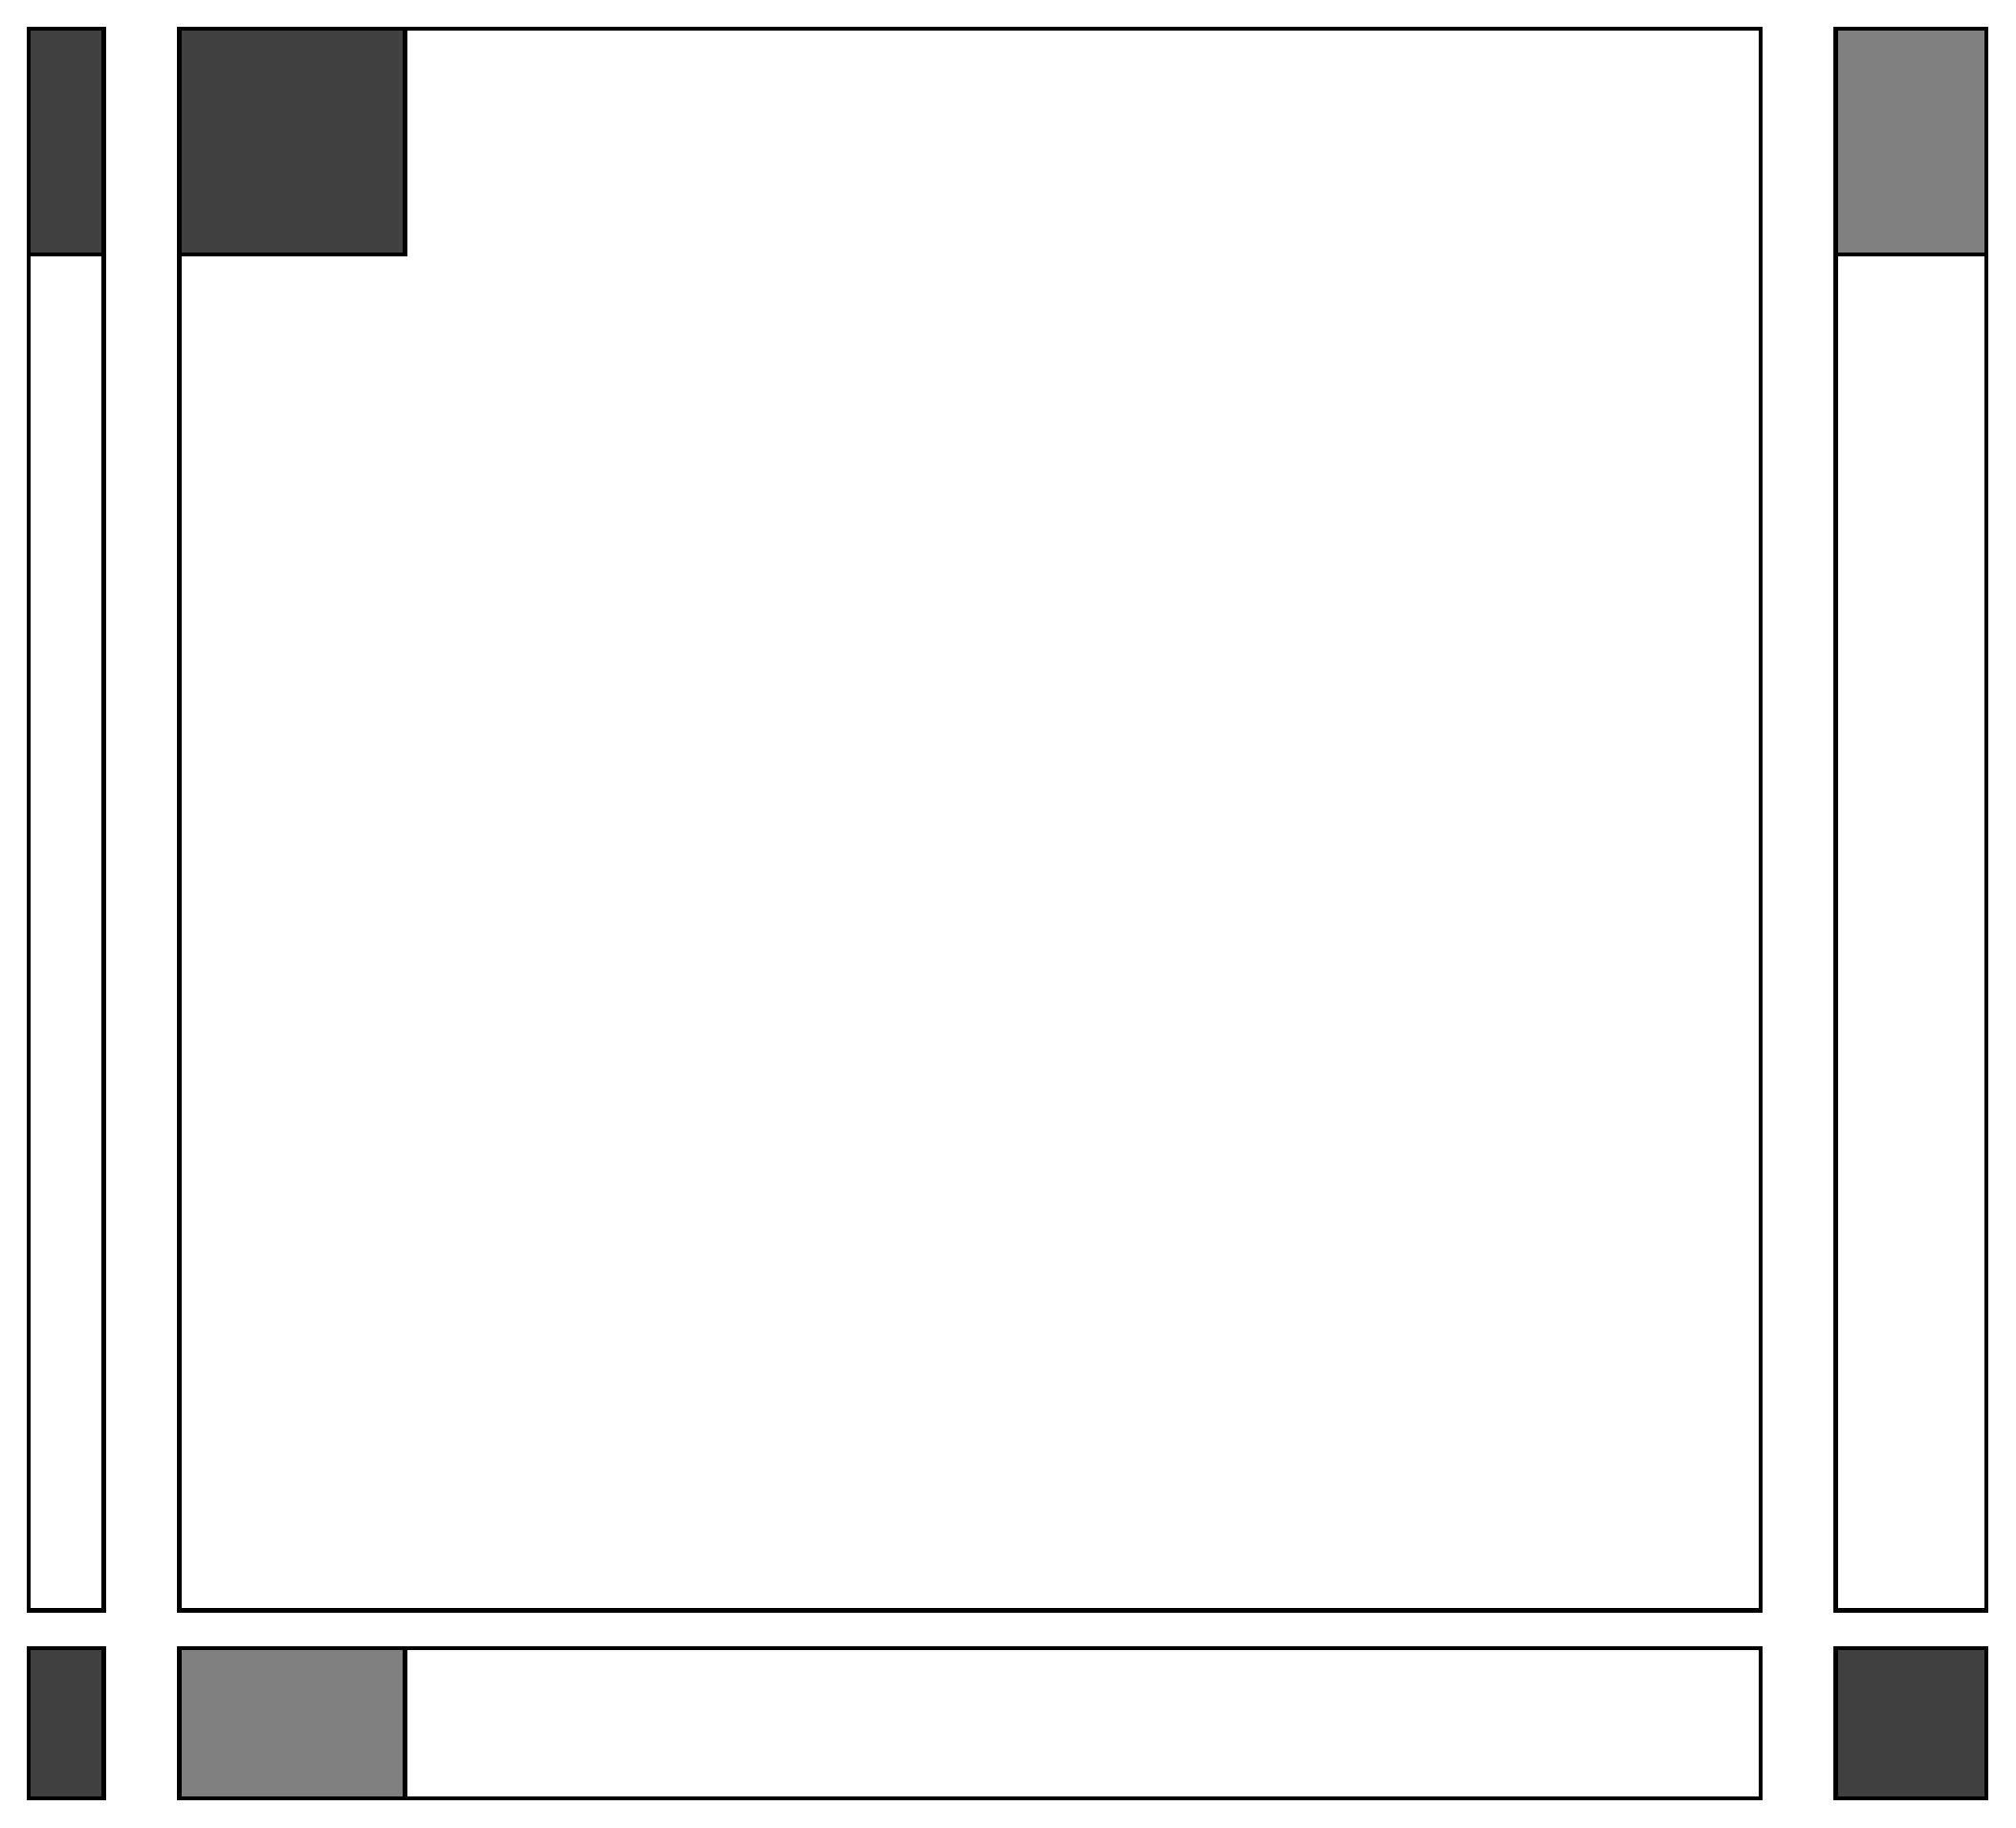
\begin{tikzpicture}
  \tikzmath{\m = 21;}
  \draw[ultra thick] (0, 2.5) rectangle ++(1, \m);
  \draw[ultra thick, fill=darkgray] (0, 2.5+\m-3) rectangle ++(1, 3);
  \draw[ultra thick, fill=darkgray] (0, 0) rectangle ++(1, 2);


  \draw[ultra thick] (2, 2.5) rectangle ++(\m, \m);
  \draw[ultra thick, fill=darkgray] (2, 2.5+\m-3) rectangle ++(3, 3);
  
  \draw[ultra thick] (2, 0) rectangle ++(\m, 2);
  \draw[ultra thick, fill=gray] (2, 0) rectangle ++(3, 2);

  \draw[ultra thick] (2.5+\m+0.5, 2.5) rectangle ++(2, \m);
  \draw[ultra thick, fill=gray] (2.5+\m+0.5, 2.5+\m-3) rectangle ++(2, 3);
  \draw[ultra thick, fill=darkgray] (2.5+\m+0.5, 0) rectangle ++(2, 2);
\end{tikzpicture}
\end{document}